Differences in gender are central features of economic and social life. This paper investigates how participation in enriched early childhood programs differently enhances the lives of disadvantaged boys and girls, and whether they enhance or reduce lifetime gender gaps among disadvantaged children.

There is a rich literature in psychology on the greater vulnerability of boys to adverse life conditions. As a group, girls mature earlier, are more resilient to adversity, and perform better in a variety of life tasks.\footnote{See \cite{Schore_2017_IMHJ} for an extensive survey of this literature. Economists have contributed to this literature. See, e.g., \cite{Autor-etal_2015_Family-Disadvantage}.} Less is known about effective strategies for reducing the vulnerability of boys to disadvantage. 

This paper investigates this question using data from a randomized controlled trial of a prototypical intensive early childhood program that enriched the early lives of disadvantaged children. The program is a template for many current and proposed early interventions. It starts at eight weeks of age and continues through age 5. Participants and controls are followed through age 34 with data collected at all stages of the life cycle.

There are positive life-cycle impacts of the program for both genders. However, there are substantial differences in impact by gender that vary by domain. The program studied differentially promotes the earnings, employment and health of males and reduces their participation in crime. It differentially enhances the IQ, cognition and educational attainment of girls. 

We investigate the sources of these differences. Boys placed in childcare benefit relatively more from high quality center care (compared to low-quality childcare) than girls, although both genders benefit. This is consistent with a large body of work in psychology on vulnerability and the importance of early attachment on the lives of boys. 

We analyze data from the Carolina Abecedarian Project (ABC) and its closely aligned sister program, Carolina Approach to Responsive Education (CARE). These programs were conducted in Chapel Hill, North Carolina for a sample of children born between 1972 and 1980. We refer to the combined programs as ABC/CARE.

To preview of our analysis, we report gender differences of outcomes in Figure~\ref{fig:proportion}. We report the proportion of outcomes, by category, for which the males outperform the females (we explain these outcomes in greater detail in the main body of the paper). We do this for the control group and the treatment group separately to establish a baseline gender difference and the value-added of treatment. Control males have higher IQ scores, employment, parental income, and crime than females. They also do better when aggregating across all outcome categories. Treatment drastically narrows the gap between males and females for achievement, with all achievement measures favoring females in the treatment group. Education is another outcome category for which treatment narrows the gender gap. Male controls have higher educational attainment in the control group with over 50\% of the education outcomes favoring males, although the result is not statistically significant. In the treatment group, however, less than 25\% of the educational outcomes favor males. This pattern also appears for employment outcomes and grouping across all outcome categories. 

\begin{figure}[!htbp]
\centering
\caption{Proportion of Outcomes Males $>$ Females, by Outcome Category}
\label{fig:proportion}
	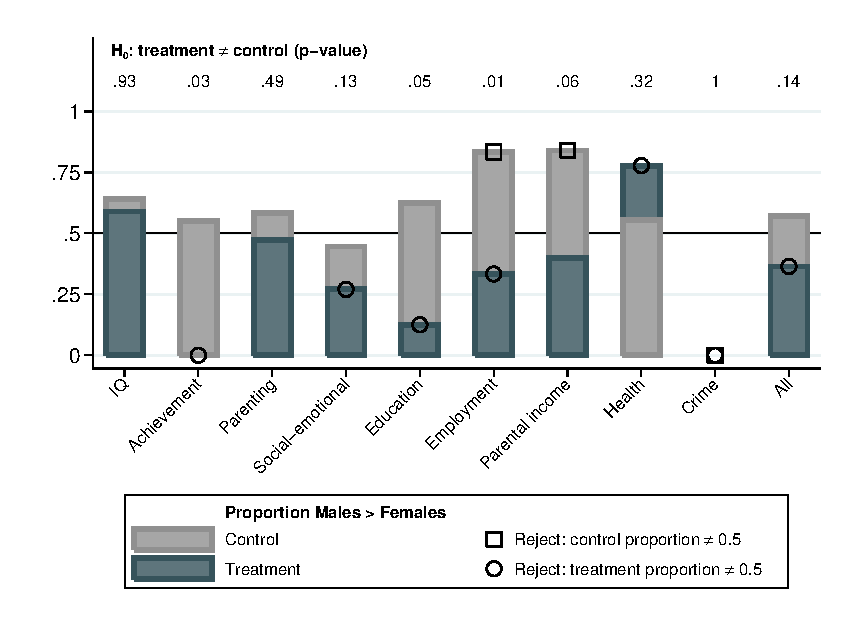
\includegraphics[width=\textwidth]{output/gendergaps-treat-vs-fullcontrol}
\footnotesize \justify
Note: These plots show the proportion of outcomes, by outcome category, for which the males' mean is larger than the females' mean. The standard errors and the $p$-values are computed using 200 bootstraps. The $p$-values are one-sided and test the null hypothesis that the proportion of outcomes is greater than $\frac{1}{2}$ The crime outcomes are all coded so that a higher value indicates more criminal activity. All other outcome categories have higher values corresponding to socially desirable outcomes. The variables for each outcome category are listed in Appendix~\ref{appendix:gdiff-outcome-list}.
\end{figure}

Table~\ref{tab:proportion-table} summarizes the gender gaps in these plots as well as those when considering the alternative setting of the control-group children. In the control group, the proportions of outcomes for which males do better than females is higher than $\frac{1}{2}$ for most of the categories, although by no means are all statistically significant. Exceptions include social-emotional skills, in which females surpass males, and crime, in which the outcomes are coded such that higher values correspond with less criminal activity. \textbf{[JJH: Code crime a positive!][This is implemented.]} Treatment reverses the gaps for achievement, education, employment, parental income, and over all outcomes. It widens the gap for health, with treatment leading males to achieve better health outcomes. Considering control-group subjects who stay at home, females have better health outcomes and commit more crimes. Both outcomes are reduced with treatment \textbf{[JJH: Why worse health?]}. Finally, the males who attend lower-quality alternative preschools do not outperform females on any of the outcome categories associated with cognition, education, and parenting. This indicates an early-life disadvantage that enriched early childcare programs partially correct.

\begin{table}[H]
\centering
\caption{Summary of Proportion of Outcomes Males $>$ Females}
\label{tab:proportion-table}
\begin{threeparttable}
\begin{tabular}{l | c |c |c| c}
\toprule
& (1) & (2) & (3) & (4) \\
Category & Control Group  &  Control Group &  Control Group &  Treatment \\
	&				&	Stay at Home		& Alternative Preschool &  Group \\
\midrule  
IQ 								& \checkmark &  \checkmark* & $\times$&\checkmark \\
Achievement						& \checkmark &  \checkmark* &$\times$ & $\times$* \\
Parenting							& \checkmark&  \checkmark* &$\times$ & \checkmark \\
Social-emotional					& $\times$&$=$ &$\times$* &$\times$* \\
Education							& \checkmark&\checkmark & $=$ &$\times$* \\
Employment						&  \checkmark* &  \checkmark* &  \checkmark* &$\times$* \\
Parental income					&  \checkmark* &\checkmark & \checkmark & $\times$\\
Health 							& \checkmark &$\times$ &\checkmark &  \checkmark* \\
Crime							&  \checkmark* &  $=$ & \checkmark* &  \checkmark* \\
\midrule
All								&  \checkmark* &\checkmark*&  $\times$ & $\times$\\
\bottomrule
\end{tabular}
\begin{tablenotes}
\footnotesize
\item Note: This table summarizes comparison of gender gaps across outcome categories by different groups. A \checkmark indicates that the proportion of outcomes in the corresponding category is larger than $\frac{1}{2}$, meaning that males outperform females. A \checkmark* indicates that the proportion is significantly larger than $\frac{1}{2}$. A $\times$ indicates that the proportion is less than $\frac{1}{2}$. A $\times$* indicates that it is significantly less than $\frac{1}{2}$. Column (1) is the difference between males and females in the full control group.  Column (2) is the difference between males and females in the control group only considering those who stayed at home. Column (3) is the difference between males and females in the control group only considering those who attended alternative preschools. Column (4) is the difference between males and females in the treatment group. The variables for each outcome category are listed in Appendix~\ref{appendix:gdiff-outcome-list}.
\end{tablenotes}
\end{threeparttable}
\end{table}

Many studies have shown the potential for early-life interventions to improve the skills of children, especially those from disadvantaged families.\footnote{\citet{Currie_2011_AER,Elango_Hojman_etal_2016_Early-Edu}.} Several of these studies report effects by gender and find that males and females differently benefit from early childhood education. For example, \citet{Heckman_Moon_etal_2010_QE} and \citet{Garcia_Heckman_Leaf_etal_2017_Comp_CBA_Unpublished}, analyze randomized controlled trials with long-term data follow-ups, and find that intervening early in life more positively affects education for females and labor market and health outcomes for males. Other studies analyzing programs with shorter-term follow-up also find similar patterns of gender differences in early skills and academic outcomes.\footnote{\citet{Deming_2009_AEJAE,Ou_Reynolds_2010_Mechanisms_CYSR,Magnuson_Kelchen_Duncan_etal_2016_ECRQ}.} None of these studies have examined the gender gap and how treatment alters it.

This paper reports the treatment effects of ABC/CARE by gender. We report treatment effects comparing treated outcomes with different control conditions, including staying at home or attending other center-based care that was of lower quality than the ABC/CARE program.\footnote{Historical documentation, records, and evidence from knowledgeable individuals indicate that although these alternate centers followed state and federal standards, they were of lower quality than the ABC/CARE program.} Unlike previous studies, we compute treatment effects comparing the treatment group to the control group fixing those in the control group to these two alternate counterfactuals (shown in Figure~\ref{fig:proportion}).\footnote{Previous studies presenting treatment effects of ABC and CARE include \citet{Ramey_etal_1985_Project-CARE_TiECSE, Clarke_Campbell_1998_ABC_Comparison_ECRQ,Campbell_Pungello_etal_2001_DP,Campbell_Ramey_etal_2002_ADS,Campbell_Wasik_etal_2008_ECRQ,Campbell_Conti_etal_2014_EarlyChildhoodInvestments}.}$^,$\footnote{See \cite{Heckman_1992_randomization}, \cite{Heckman_Hohmann_etal_2000_QJE}, and \cite{Kline_Walters_2016_QJE} for work related to control substitution.} Home care is beneficial for boys. 

This paper unfolds in the following way. In Section~\ref{sec:data}, we describe the experimental data and its special features. We document that a considerable proportion of the control group children attend lower (than treatment) preschools. In Sections~\ref{sec:parameters} and~\ref{sec:combining-functions} we define the treatment effects estimated. Section~\ref{sec:treatment-effects} reports the treatment effects overall and by gender and establish the existence of sharp gender effects in many categories of outcomes. Section~\ref{sec:gender-differences} discusses differences in the proportions of outcomes favoring men by category. Section~\ref{sec:conclusion} discusses the sources of these differences.


%ee \citet{Beeghly-etal_2017_IMHJ,Dayton_2017_IMHJ,Iruka_2017_IMHJ,Schore_2017_IMHJ} for recent findings on the topic of different development of males and females early in life. 